\documentclass{beamer}
% The graphics package
\usepackage{graphicx}
% Allows for symbols in lists
\usepackage{amssymb}


%%%%%%%% Title %%%%%%%%%%%%%%%%%%%%%%%%%%%%%%%%%%%%%%%%%%%%%%%%%%%%%%%%%%%%%%%%%
\title{Package Manager}
\subtitle{Team Figjam}
\author{\fontsize{10}{1}\selectfont
        Merrick Heley
        \and
        Tony Lee
        \and
        Nathan Woodrow
        \and
        Steven Eggington
        }
\institute{DECO2800 - Design Computing Studio 2}
\date{9 September 2013}


%%%%%%%% Notes, commands, settings %%%%%%%%%%%%%%%%%%%%%%%%%%%%%%%%%%%%%%%%%%%%%

% Set the theme for the presentation
\usetheme{Frankfurt}

%%%%%%%% Start document %%%%%%%%%%%%%%%%%%%%%%%%%%%%%%%%%%%%%%%%%%%%%%%%%%%%%%%%
\begin{document}

% Title frame
\begin{frame}
    \titlepage
\end{frame}

\begin{frame}
    \frametitle{What are you trying to achieve?}
    
    This is a really long line of text isn't it baa hahahh ahahah a hhah haha
    \\
    
    \begin{columns}
        \column{.5\textwidth}
            Text for your first column
        \column{.5\textwidth}
            Text for your second column
    \end{columns}
    
\end{frame}

\begin{frame}
    \frametitle{How are you going about it?}
    
    \begin{block}{Block title}
        This is a block in blue
    \end{block}
\end{frame}

\begin{frame}
    \frametitle{Logical Architecture}
    
    \begin{figure}[!hbp]
        \centering
        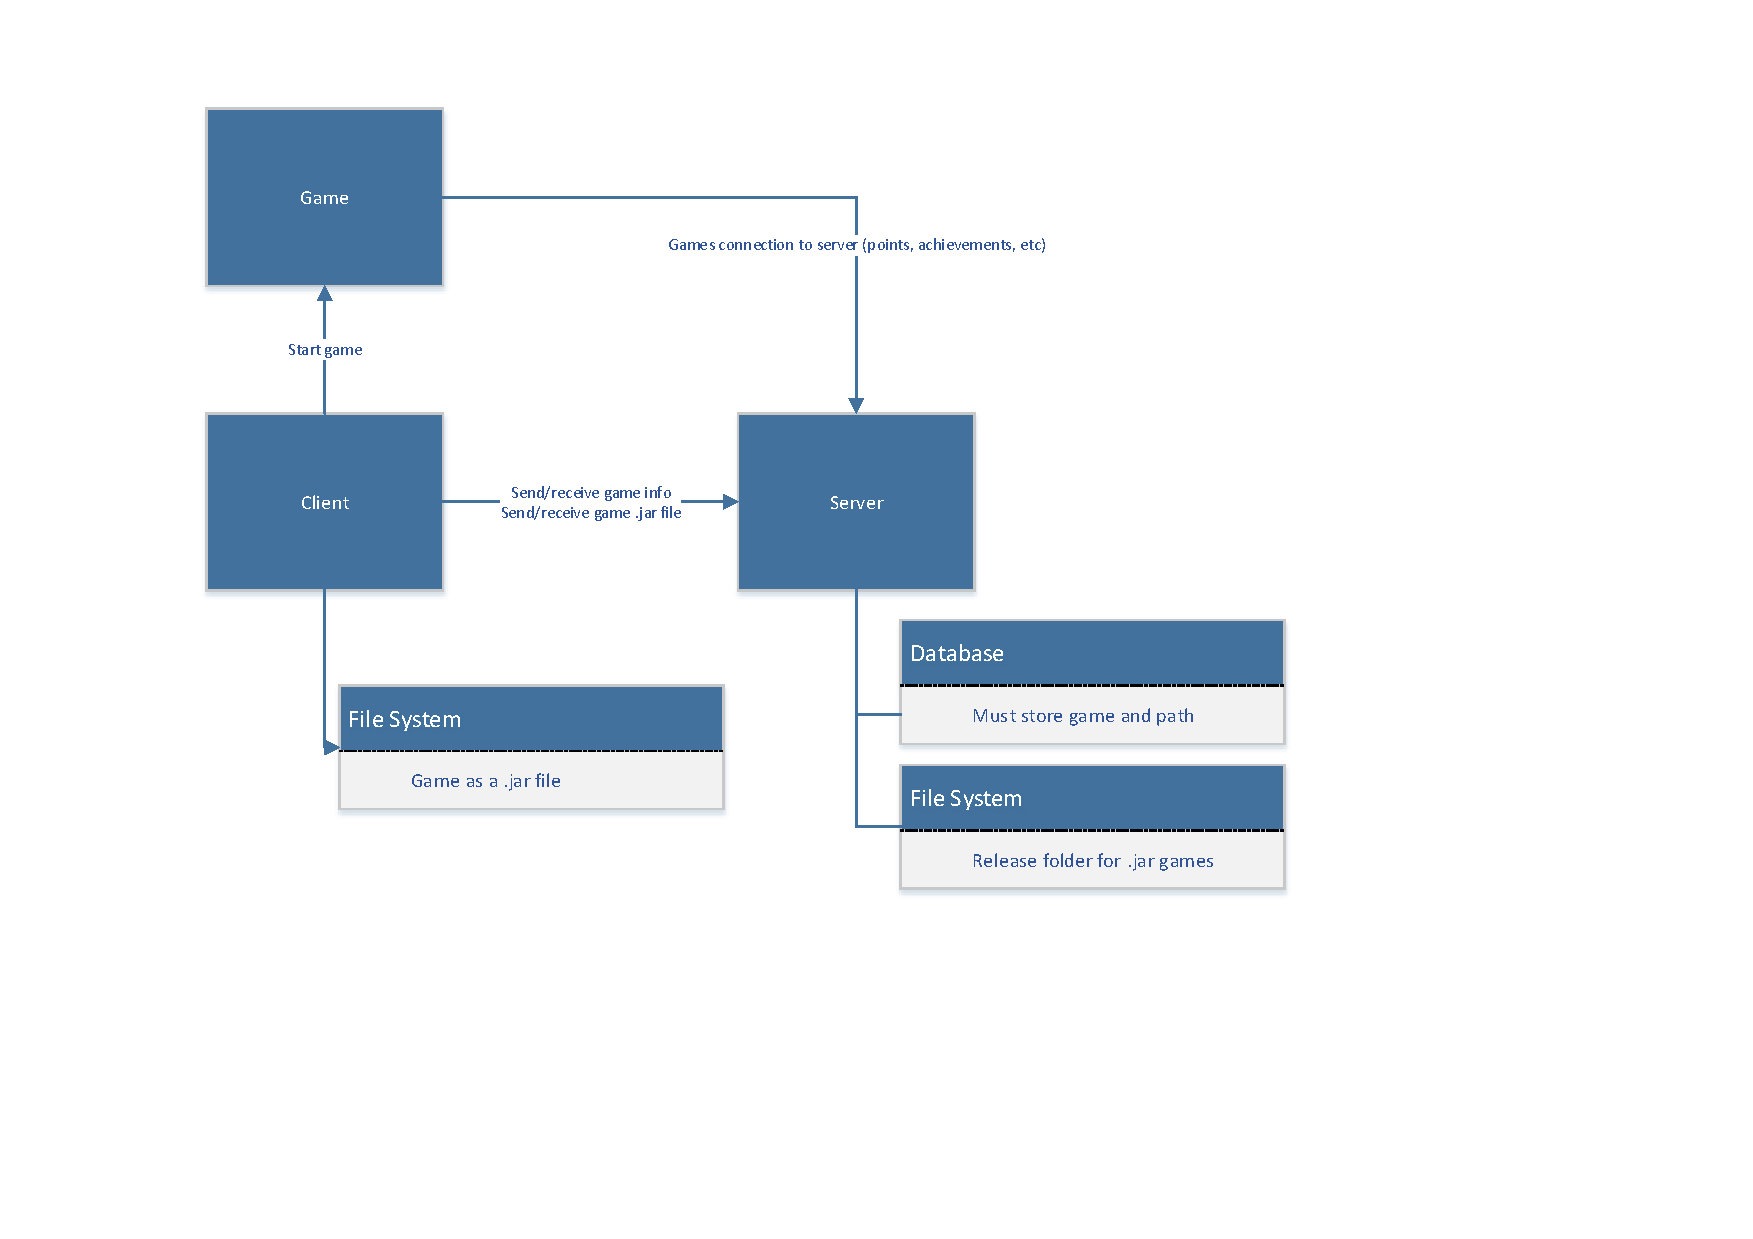
\includegraphics[trim=3cm 5cm 5cm 2cm,
                         clip=true,
                         width=\textwidth]{logarch.pdf}
    \end{figure}
    
\end{frame}

\begin{frame}
    \frametitle{How is it coming along?}
    
    \begin{block}{Block title}
        This is a block in blue
    \end{block}
\end{frame}

\begin{frame}
    \frametitle{Feedback}
    
    \begin{block}{Block title}
        This is a block in blue
    \end{block}
\end{frame}


\end{document}